\documentclass[11pt,a4paper]{article}

\usepackage[margin=1in]{geometry}
\usepackage{graphicx}
\usepackage{booktabs}
\usepackage{amsmath}
\usepackage{hyperref}
\usepackage{float}
\usepackage{caption}
\usepackage[T1]{fontenc}
\usepackage{lmodern}
\usepackage{microtype}
\usepackage{xcolor}
\usepackage{enumitem}
\usepackage{subcaption}

\graphicspath{{../data/analysis/}{../data/analysis_sbert/}}

\title{\textbf{Plurality Collapse: Measuring the Dimensionality Gap\\Between Human and LLM Moral Reasoning}}
\author{Xan Carey}
\date{April 2026}

\begin{document}
\maketitle

\begin{abstract}
We embed human and LLM rationales from 10,826 everyday moral dilemmas into the Kaleido-XL moral knowledge encoder (2048-dim) and measure the geometric dimensionality of each source's embedding distribution. Human rationales require 448 PCA components for 90\% variance explanation compared to 317--332 for seven LLMs at matched sample sizes---a 35--41\% dimensionality gap. Cross-space projection confirms the gap is asymmetric: human principal components capture 87\% of LLM variance, but LLM principal components capture only 82\% of human variance. Using Kaleido's decoder to qualify the residual stream, we show the extra dimensions encode genuinely diverse moral values (Pearson $r = 0.935$ between reconstruction error and value diversity), not stylistic noise. The gap persists in a general-purpose Sentence-BERT encoder (768-dim) with proportionally similar magnitude, is uniform across consensus levels, and is invisible to categorical analysis---silhouette scores of 0.02--0.04 confirm the moral value space is a continuum, not a taxonomy.
\end{abstract}

%% ============================================================================
\section{Introduction}
%% ============================================================================

Do large language models flatten the diversity of human moral reasoning? When LLMs generate rationales for everyday moral dilemmas, do they capture the same breadth of moral perspectives that humans express, or do they collapse a high-dimensional space of values, framings, and situational judgments into a lower-dimensional subspace?

This question matters because LLMs are increasingly deployed in contexts that require moral reasoning---content moderation, advisory systems, ethical review tools. If LLMs systematically underrepresent certain moral perspectives, their outputs will reflect a narrower value system than the populations they serve. The concern is not that LLMs produce \emph{wrong} moral judgments, but that they produce \emph{insufficiently diverse} ones, missing the plurality of legitimate moral viewpoints that characterizes genuine human discourse.

We operationalize ``diversity of moral reasoning'' as the geometric dimensionality of rationale embeddings in a moral knowledge representation space. Our analysis proceeds in six layers: (1) establishing that a dimensionality gap exists between human and LLM rationale embeddings, (2) showing the gap is asymmetric---human principal components explain LLM variance better than the reverse, (3) qualifying what the extra dimensions contain by decoding the residual stream, (4) characterizing the resulting frequency distortion across the full moral vocabulary, (5) showing the compression is structural rather than context-dependent, and (6) demonstrating that the moral value space is fundamentally continuous, resisting categorical analysis.

%% ============================================================================
\section{Data and Embedding}
%% ============================================================================

\subsection{Dataset}

We use the Sachdeva et al.\ \emph{Normative Evaluation of LLMs on Everyday Dilemmas} dataset, which contains 10,826 moral dilemmas from Reddit's ``Am I the Asshole'' forum. Each dilemma includes the original post, a top human comment (rationale), and moral rationales generated by seven LLMs: GPT-3.5, GPT-4, Claude, Bison, Gemma, Mistral, and Llama. Each LLM provides 2--3 rationales per dilemma (yielding 21,652--32,478 LLM rationales per model, 216,497 total). The dataset also provides weighted community agreement scores across four verdict categories (NTA, YTA, ESH, NAH).

\subsection{Embedding}

We encode all rationales using Kaleido-XL, an encoder-decoder model trained on ValuePrism---a dataset of 31,000 human-written situations annotated with GPT-4-generated moral values (filtered by human validators)---to map natural language to moral value expressions. Each rationale is formatted with Kaleido's generation template and passed through the encoder; final hidden states are mean-pooled, producing a 2048-dimensional embedding per rationale. This encoder was chosen because its representation space is explicitly structured around moral knowledge, making dimensionality in this space a meaningful proxy for moral reasoning diversity.

Kaleido-XL is an encoder-decoder architecture: the encoder produces the 2048-dim embeddings that form our primary data; the decoder can generate moral value labels from those embeddings, which we use beginning in Layer 3 to qualify what the dimensionality gap contains. Each subsequent layer describes its own analysis methods and robustness checks inline.

%% ============================================================================
\section{Layer 1: A Dimensionality Gap Exists}
%% ============================================================================

We begin with the raw geometric question: do human and LLM rationale embeddings occupy the same number of effective dimensions?

\paragraph{Method.} For each source, we fit full PCA on the embedding matrix and compute two complementary dimensionality measures. (1) \emph{Participation ratio} PR $= (\sum \lambda_i)^2 / \sum \lambda_i^2$: the effective number of dimensions that carry variance. If all variance concentrates in 1 dimension, PR $= 1$; if it spreads evenly across $d$ dimensions, PR $= d$. PR is sensitive to the bulk of the eigenvalue distribution. (2) \emph{Components for 90\%/95\% variance}: the number of principal components $k$ such that cumulative explained variance reaches the threshold. Unlike PR, this metric captures the long tail of small eigenvalues, making it sensitive to rare-but-nonzero directions of variation. Sources are: human, each of the seven individual LLMs, and ``all LLM''---the vertical concatenation of all seven LLM embedding matrices into a single $216{,}497 \times 2048$ matrix. This pooled source represents the collective LLM distribution: the moral reasoning subspace that the seven models jointly span. Analyzing it alongside individual models tests whether the dimensionality gap is a property of LLMs as a class rather than of any single model.

\subsection{The Gap}

\begin{table}[H]
\centering
\caption{PCA dimensionality metrics per source (full sample sizes, Kaleido-XL).}
\label{tab:summary}
\begin{tabular}{lrrrrr}
\toprule
Source & $n$ & PR & Kernel PR & Comp.\ 90\% & Comp.\ 95\% \\
\midrule
Human   & 10,826  & 52.40 & 52.92 & \textbf{448} & \textbf{785} \\
GPT-3.5 & 32,478  & 49.76 & 52.41 & 329 & 642 \\
GPT-4   & 21,652  & 54.36 & 56.70 & 341 & 658 \\
Claude  & 32,478  & 52.06 & 54.17 & 340 & 653 \\
Bison   & 32,478  & 52.00 & 53.78 & 336 & 652 \\
Gemma   & 32,478  & 46.16 & 48.62 & 334 & 653 \\
Mistral & 32,455  & 42.65 & 45.82 & 332 & 654 \\
Llama   & 32,478  & 51.08 & 53.25 & 333 & 651 \\
All LLM & 216,497 & 51.95 & 54.19 & 347 & 679 \\
\bottomrule
\end{tabular}
\end{table}

Human rationales require 448 components for 90\% variance, compared to 329--341 for individual LLMs and 347 for the combined pool. The cumulative variance curves (Figure~\ref{fig:cumvar}) make the gap visible: human variance accumulates more slowly, with a longer tail extending past the point where LLM curves have already flattened.

\begin{figure}[H]
\centering

\includegraphics[width=\textwidth]{cumulative_variance.png}
\caption{Cumulative explained variance by number of PCA components. Annotated dots mark the 90\% and 95\% thresholds for human and all-LLM. Human reaches 90\% at $k = 448$ and 95\% at $k = 785$; all-LLM at $k = 347$ and $k = 679$. The gap widens steadily through the tail.}
\label{fig:cumvar}
\end{figure}

The participation ratio is less sensitive to this gap (human PR $= 52.40$ vs.\ LLM range $42.65$--$54.36$) because PR is dominated by the top eigenvalues. The components-for-90\% metric captures the ``long tail'' where human reasoning extends into dimensions LLMs do not use.

\subsection{Robustness}

Four alternative explanations could account for the dimensionality gap without invoking genuine differences in moral reasoning diversity. We test and rule out each.

\paragraph{Sample size.} The most immediate confound: LLM sources have 2--3$\times$ more rationales than human (21,652--32,478 vs.\ 10,826). More data points mechanically increase the number of PCA components needed to explain a fixed variance threshold, because additional samples can populate directions that smaller samples leave empty. Beyond the count difference, each LLM provides 2--3 rationales per dilemma, while human data has exactly 1. Within-dilemma rationales respond to the same prompt and are therefore correlated, which could deflate LLM dimensionality and inflate the gap.

We test two subsampling strategies. First, random subsampling: draw $n = 10{,}826$ rationales uniformly from each LLM's pool (5 seeds). LLMs range from 317.0 (GPT-3.5) to 332.2 (GPT-4) components for 90\% variance, yielding a \textbf{35--41\%} gap against the human 448. Second, dilemma-matched subsampling: for each of the 10,826 dilemmas, randomly select exactly 1 of the LLM's 2--3 runs, matching the human data structure exactly. This shifts comp90 upward by only 2--5 components (range 319.8--334.0), narrowing the gap to \textbf{34--40\%}. A cross-model variant---selecting 1 rationale per dilemma from any of the 7 LLMs---yields comp90 $= 329.6 \pm 0.8$, a 35.9\% gap. Under both strategies, each LLM's comp90 varies by less than 1 component across seeds (std $< 1$), and the human--LLM gap of 114--131 components exceeds 100$\times$ this subsampling noise (Figure~\ref{fig:subsample}).

\begin{figure}[H]
\centering
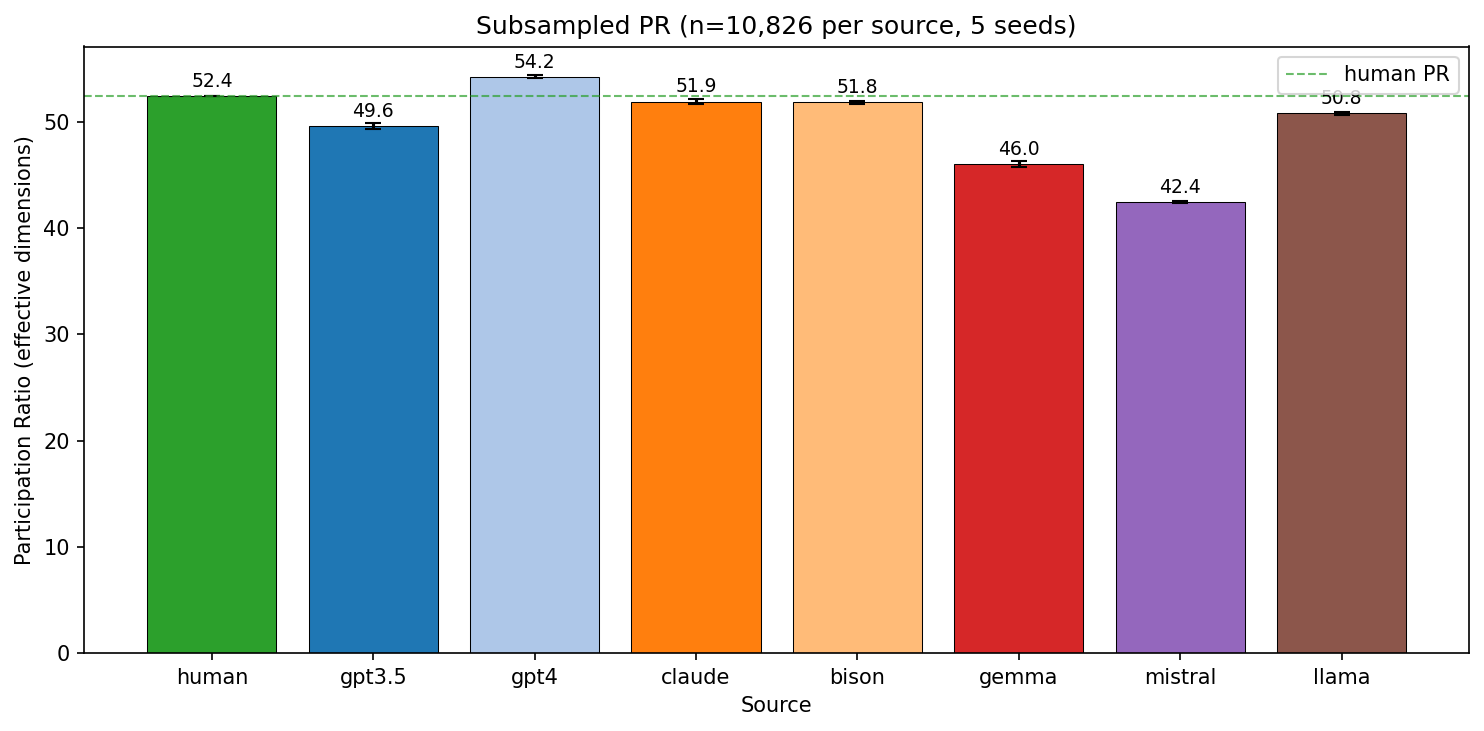
\includegraphics[width=0.85\textwidth]{subsample_pr_comparison.png}
\caption{Participation ratio at matched sample sizes ($n = 10{,}826$, 5 seeds). Error bars show $\pm 1$ std across seeds.}
\label{fig:subsample}
\end{figure}

\paragraph{Text length.} Human rationales average 57.2 words; LLM rationales average 94.4 words (range 67--135 across models). Longer text could produce higher-dimensional embeddings simply by containing more information per rationale, regardless of moral content. We test this by binning all rationales into word-count quintiles and computing PCA within each bin, so that human and LLM rationales of the same length are compared directly. Quintile boundaries (23, 35, 52, 81 words) are the 20th--80th percentiles of the human word-count distribution, ensuring balanced human bins; the same boundaries are applied to LLM rationales. Within each bin, both sources are subsampled to matched $n$ (the smaller of the two counts, capped at 2,000) to eliminate any residual sample-size confound.

\begin{table}[H]
\centering
\caption{PCA metrics by word-count quintile at matched $n$ within each bin.}
\label{tab:length_quintile}
\begin{tabular}{lrrrrr}
\toprule
Quintile & $n$ (matched) & Human comp90 & LLM comp90 & Gap & Gap \% \\
\midrule
Q0 ($<$23 words) & 477   & 192 & 131 & 61  & 47\% \\
Q1 (23--35)       & 2,000 & 362 & 256 & 106 & 41\% \\
Q2 (35--52)       & 2,000 & 365 & 263 & 102 & 39\% \\
Q3 (52--81)       & 2,000 & 364 & 266 & 98  & 37\% \\
Q4 ($>$81 words)  & 2,000 & 349 & 269 & 80  & 30\% \\
\bottomrule
\end{tabular}
\end{table}

The gap persists within every length bin at matched $n$ (Table~\ref{tab:length_quintile}): 80--106 extra components in Q1--Q4, comparable to the 114--131 gap in the full-sample analysis. Q0 has only 477 LLM rationales (most LLM output exceeds 23 words), mechanically depressing both sources' comp90 but preserving a 47\% gap. Text length does not explain the dimensionality difference.

\paragraph{Nonlinearity.} PCA assumes that meaningful variation lies along linear subspaces. If the embedding distributions have nonlinear structure---e.g., curved manifolds that PCA mischaracterizes as high-dimensional---then the gap could reflect a geometric artifact of the linear method rather than genuine distributional differences. Kernel PCA with an RBF kernel captures nonlinear structure by implicitly mapping to a higher-dimensional feature space.

Linear and kernel PR are near-identical across all 9 sources (Pearson $r = 0.984$, $p < 10^{-6}$), with a mean absolute difference of 2.16 and a maximum shift of 3.17 (Mistral). The two methods produce effectively the same ranking of sources and the same gap structure, indicating that the Kaleido embedding space does not contain nonlinear structure that linear PCA mischaracterizes.

\paragraph{Distillation bias.} Kaleido-XL was trained on ValuePrism, a dataset of 218,000 values, rights, and duties connected to 31,000 human-written situations. The situations are human-authored, but the value annotations Kaleido is fine-tuned on were generated by GPT-4. Kaleido's encoder has therefore learned to represent moral reasoning through the lens of GPT-4's value generation patterns. If this distillation biases the encoder to represent LLM-style reasoning more efficiently than human reasoning, the dimensionality gap could reflect encoder bias rather than genuine diversity differences. A general-purpose encoder with no moral-specific training should not share this particular bias, though it may introduce its own from pretraining corpus composition.

We replicate the full PCA analysis using Sentence-BERT (\texttt{all-mpnet-base-v2}, 768-dim). The dimensionality gap persists with proportionally similar magnitude for every individual model (Table~\ref{tab:kaleido_sbert}). An encoder that has never seen GPT-4 moral value training data detects the same structural difference in the principal components of rationale embeddings.

\begin{table}[H]
\centering
\caption{Kaleido vs.\ SBERT dimensionality comparison (matched $n = 10{,}826$).}
\label{tab:kaleido_sbert}
\begin{tabular}{lrrrr}
\toprule
Source & Kaleido comp90 & SBERT comp90 & Kaleido PR & SBERT PR \\
\midrule
Human   & 448   & 202   & 52.40 & 76.46 \\
GPT-3.5 & 317.0 & 152.2 & 49.60 & 50.91 \\
GPT-4   & 332.2 & 159.0 & 54.23 & 50.40 \\
Claude  & 328.0 & 143.8 & 51.88 & 52.69 \\
Bison   & 324.2 & 161.2 & 51.82 & 55.49 \\
Gemma   & 321.8 & 146.0 & 46.02 & 44.64 \\
Mistral & 319.6 & 158.0 & 42.43 & 57.09 \\
Llama   & 322.0 & 143.0 & 50.80 & 54.45 \\
\midrule
All LLM & 347   & 158   & 51.95 & 51.52 \\
\bottomrule
\end{tabular}
\end{table}

%% ============================================================================
\section{Layer 2: The Gap Is Asymmetric}
%% ============================================================================

Layer 1 shows that human rationales occupy more dimensions, but not whether those extra dimensions overlap with LLM dimensions. We distinguish these by projecting each source's data onto the other source's principal components.

\subsection{Cross-Space Projection}

Human principal components($k = 448$) capture 87.3\% of all-LLM variance whereas all-LLM principal components($k = 347$) capture 81.6\% of human variance---an asymmetry of $+5.7$ percentage points (Figure~\ref{fig:cross_curves}).

\begin{figure}[H]
\centering
\includegraphics[width=0.85\textwidth]{cross_projection_curves.png}
\caption{Variance captured when projecting one source's data onto the other source's principal components. Human principal components capture more LLM variance (green) than LLM principal components capture human variance (pink). The gap between curves is the asymmetry ($+5.7$\%).}
\label{fig:cross_curves}
\end{figure}

\begin{figure}[H]
\centering
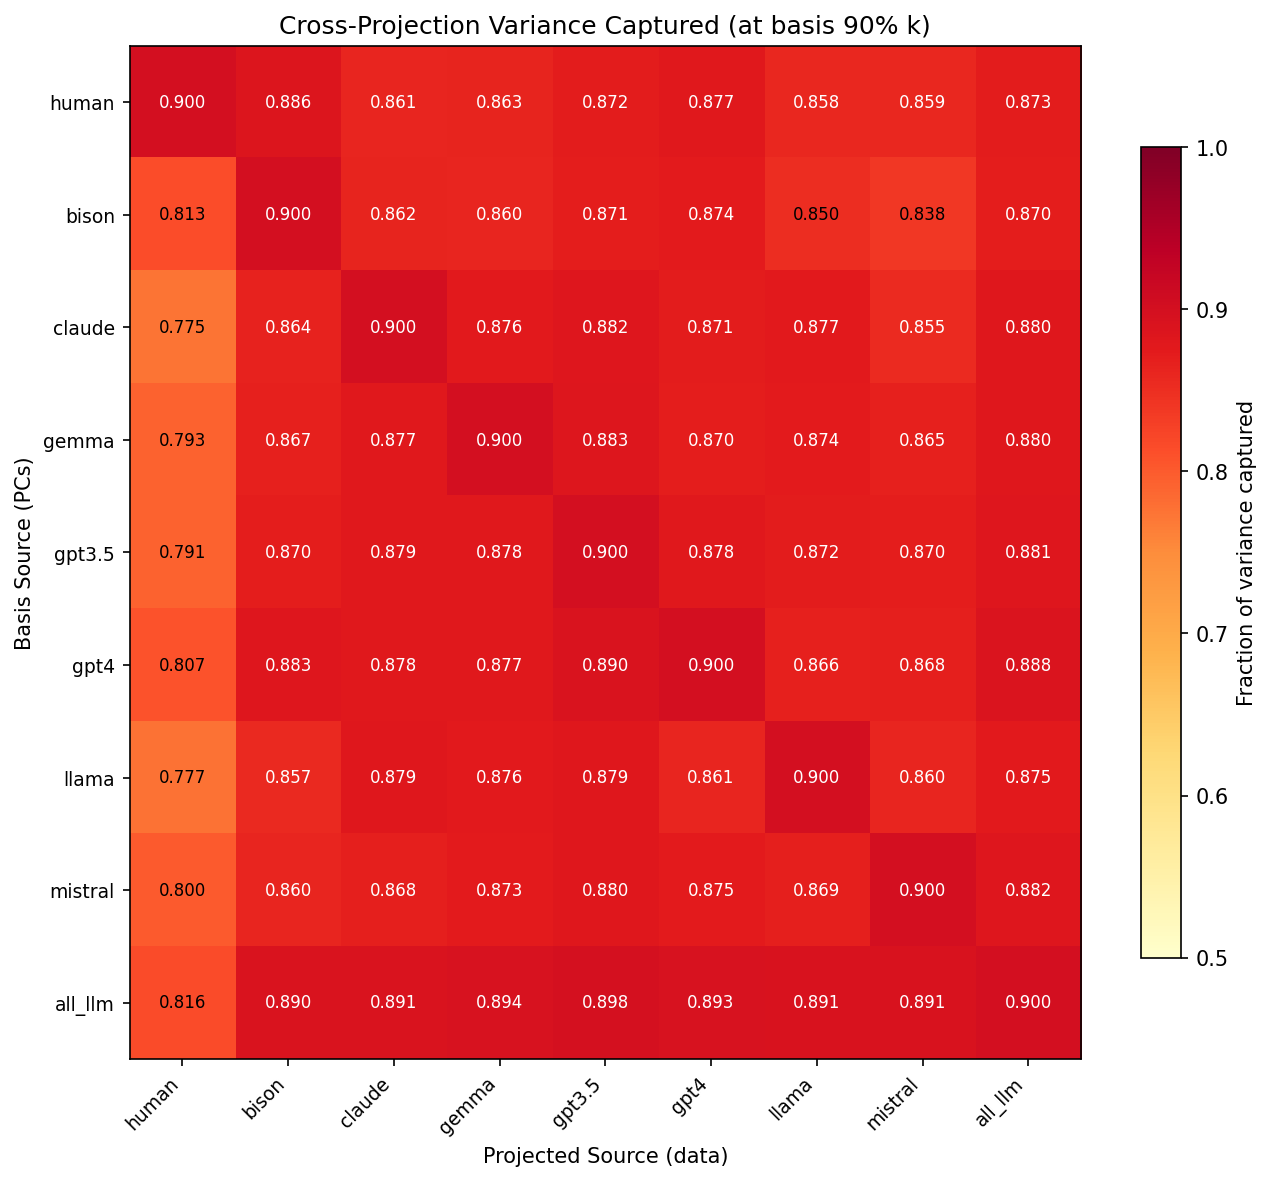
\includegraphics[width=0.78\textwidth]{cross_projection_heatmap.png}
\caption{Cross-projection heatmap (Kaleido). Rows = basis principal components, columns = projected data. Human$\to$LLM values (top row) systematically exceed LLM$\to$human values (left column).}
\label{fig:heatmap}
\end{figure}

The heatmap (Figure~\ref{fig:heatmap}) shows that LLM principal components capture only 77.5--81.3\% of human variance, while human principal components capture 85.8--87.7\% of each LLM.

\subsection{Robustness}

\paragraph{Distillation bias.} The cross-projection asymmetry is actually \emph{larger} in SBERT ($+9.4$\%: human principal components capture 89.7\% of LLM variance vs.\ 80.4\% in the reverse direction) than in Kaleido ($+5.7$\%), confirming the overlap is not encoder-specific.

\begin{figure}[H]
\centering

\includegraphics[width=0.78\textwidth]{../data/analysis_sbert/cross_projection_heatmap.png}
\caption{SBERT cross-projection heatmap. The asymmetry pattern replicates with even larger magnitude.}
\label{fig:sbert_heatmap}
\end{figure}

Thus far we've established that human rationale embeddings occupy more dimensions than LLM embeddings and that there is significant overlap in the variance of the data that the respective principal components explain. But what do these extra dimensions contain?

%% ============================================================================
\section{Layer 3: What the Extra Dimensions Contain}
%% ============================================================================

The extra dimensions could reflect genuine moral content, stylistic variation (Reddit slang, informal register), topic diversity (humans discuss a wider range of situations), or noise. When we project a rationale onto the other source's principal components and reconstruct it, the difference between the original and the reconstruction---the \emph{residual}---is the part of that rationale's representation that the other source's dimensions cannot capture. Cross-projection produces these residuals in both directions: LLM principal components leave 18.4\% of human variance unexplained, and human principal components leave 12.7\% of LLM variance unexplained. To test what these residuals contain, we use Kaleido-XL's decoder to generate a moral value label---a short string identifying the moral concept a rationale invokes---for each rationale. Since Kaleido produces near-synonyms as distinct labels (e.g., Freedom of speech, Freedom of expression, Freedom), we collapse all labels into semantic clusters throughout this section so that diversity counts reflect distinct moral \emph{concepts}, not label granularity.

\subsection{Value Diversity Gradient}

We sort all 10,826 human rationales by their residual magnitude under LLM principal components and bin them into sliding windows ($w = 200$, step $= 50$). Within each bin, we count unique value clusters and compute Shannon entropy (a measure of how evenly distributed the labels are---higher entropy means the bin's rationales spread across many values rather than concentrating in a few). If the extra dimensions encode moral content, rationales with larger residuals should produce more diverse value labels. If they encode noise or style, there should be no relationship.

\begin{figure}[H]
\centering
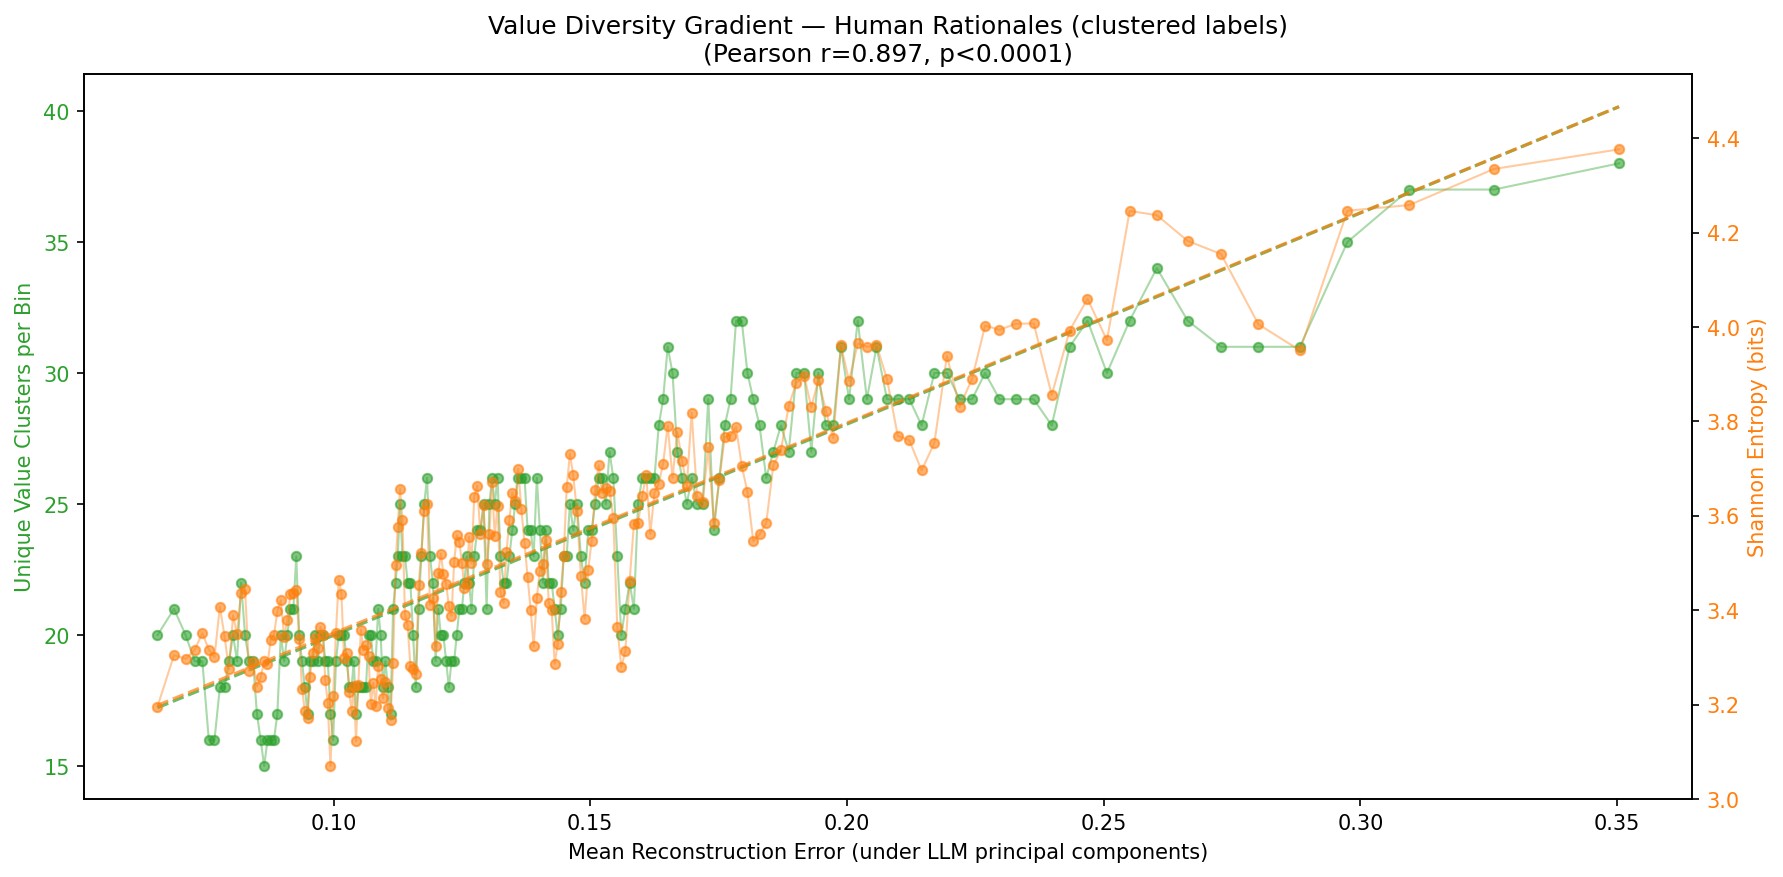
\includegraphics[width=\textwidth]{value_diversity_sliding.png}
\caption{Value diversity gradient (Kaleido, clustered labels, sliding window $w = 200$, step $= 50$). Each point is a bin of 200 rationales, ordered left-to-right by increasing reconstruction error. The green line (left axis) shows unique moral value clusters per bin; the orange line (right axis) shows Shannon entropy. Both increase monotonically ($r = 0.897$, $p < 0.0001$).}
\label{fig:gradient_kaleido}
\end{figure}

The relationship is continuous across all 10,826 rationales (Figure~\ref{fig:gradient_kaleido}). At the left edge, bins of well-captured rationales produce $\sim$15 unique value clusters; at the right edge, bins of poorly-captured rationales produce $\sim$35--38. The sliding window Pearson correlation is $r = 0.897$ ($p < 0.0001$).

The reverse gradient tells the same story. Sorting all 216,497 LLM rationales by their reconstruction error under human principal components ($k = 448$), LLM rationales that human dimensions fail to capture also invoke more diverse moral values ($r = 0.823$, $p < 0.0001$; Figure~\ref{fig:gradient_llm}). The extra dimensions on both sides encode moral content, not noise.

\begin{figure}[H]
\centering
\includegraphics[width=\textwidth]{value_diversity_llm_sliding.png}
\caption{Value diversity gradient for LLM rationales under human principal components (clustered labels, sliding window). Rationales with larger residuals invoke more diverse moral values ($r = 0.823$).}
\label{fig:gradient_llm}
\end{figure}

\subsection{Robustness}

\paragraph{Distillation bias.} All four combinations of encoder (Kaleido, SBERT) and projection direction (human under LLM, LLM under human) produce significant value diversity gradients:

\begin{table}[H]
\centering
\caption{Value diversity gradient Pearson $r$ across encoders and projection directions (clustered labels).}
\label{tab:gradient_matrix}
\begin{tabular}{lrr}
\toprule
 & Kaleido & SBERT \\
\midrule
Human under LLM principal components & 0.897 & 0.899 \\
LLM under human principal components  & 0.823 & 0.593 \\
\bottomrule
\end{tabular}
\end{table}

The human-side gradients are stronger because human residuals are larger (18.4\% vs.\ 12.7\% unexplained variance). The SBERT LLM-under-human gradient is the weakest ($r = 0.593$): in SBERT space, the human distribution has a much higher participation ratio (76.46 vs.\ 51.52 for LLMs), meaning human variance is spread diffusely across many dimensions rather than concentrated in a few structured directions. This makes the human SBERT PCA basis a less effective filter---the LLM residuals it produces are noisier and less informative about moral content specifically. In Kaleido, both sources have similar PR ($\sim$52), so both PCA bases are comparably structured. All four gradients are significant at $p < 0.0001$.

\paragraph{Stylistic confound.} TF-IDF analysis---which scores words by how distinctive they are to one group relative to another---on the surface text of poorly-captured vs.\ well-captured rationales reveals that human residuals contain stylistic markers (Reddit slang like \emph{nta}, \emph{lol}; profanity like \emph{fuck}, \emph{wtf}) alongside content terms (\emph{lawyer}, \emph{door}, \emph{service}) (Figure~\ref{fig:human_tfidf}). This confirms that Kaleido's encoder does not fully separate register from moral content. However, the value diversity gradient ($r = 0.897$) is measured via decoded moral labels, not surface text---it is independent of stylistic variation. The LLM residuals have a different character: the distinguishing terms are analytical (\emph{information}, \emph{determine}, \emph{judgment}, \emph{definitive}) rather than informal (Figure~\ref{fig:llm_tfidf}).

\begin{figure}[H]
\centering
\includegraphics[width=0.75\textwidth]{human_tfidf_terms.png}
\caption{TF-IDF terms distinguishing poorly-captured (green) from well-captured (pink) human rationales.}
\label{fig:human_tfidf}
\end{figure}

\begin{figure}[H]
\centering
\includegraphics[width=0.75\textwidth]{llm_tfidf_terms.png}
\caption{TF-IDF terms distinguishing poorly-captured (red) from well-captured (blue) LLM rationales.}
\label{fig:llm_tfidf}
\end{figure}

%% ============================================================================
\section{Layer 4: The Gap Reflects Frequency Compression}
%% ============================================================================

Layers 1--3 establish that human rationales occupy more dimensions, that the gap is asymmetric, and that the extra dimensions encode moral content. The cross-projection in Layer 2 measures variance explained along linear directions, which confirms substantial overlap (81.6\% of human variance captured) but cannot distinguish between regions that LLMs populate densely and regions they populate sparsely---a few LLM rationales in a direction are enough to create a principal component, even if that region is nearly empty. Layer 4 measures the \emph{local density} of LLM rationales around each human rationale, testing whether the dimensionality gap reflects a smooth gradient of decreasing LLM presence rather than a hard boundary.

\paragraph{Method.} To measure how densely LLMs populate different regions of the embedding space, we PCA-reduce all 227,323 raw Kaleido embeddings (human + all-LLM) to 200 dimensions (84.5\% variance explained) and use $k$-nearest neighbors ($k = 50$) in this shared space. For each human rationale, we compute: (1) the mean distance to its 50 nearest LLM neighbors, (2) the mean distance to its 50 nearest human neighbors, and (3) the ratio of these two distances. A high ratio means the rationale sits in a region where LLMs are sparse relative to humans. We then correlate these density measures with the per-rationale reconstruction errors from Layer 2.

\subsection{LLM Density Drops Where Human Residuals Are Large}

Human rationales with high reconstruction error---the ones that LLM principal components fail to capture---are farther from their nearest LLM neighbors (Pearson $r = 0.846$, $p < 10^{-300}$). The binned analysis (Figure~\ref{fig:freq_geom_binned}, sliding window $w = 200$, step $= 50$) shows this is a smooth, monotonic relationship: the mean distance to 50 nearest LLM neighbors rises steadily with reconstruction error ($r = 0.969$), while the number of LLM neighbors within a fixed radius drops ($r = -0.527$).

\begin{figure}[H]
\centering
\includegraphics[width=\textwidth]{frequency_geometry_binned.png}
\caption{LLM density around human rationales vs.\ reconstruction error (sliding window). Green (left axis): mean distance to 50 nearest LLM neighbors---increases monotonically ($r = 0.969$). Orange (right axis): mean LLM neighbors within fixed radius---decreases ($r = -0.527$). Human rationales that occupy the extra dimensions are in LLM-sparse regions of embedding space.}
\label{fig:freq_geom_binned}
\end{figure}

The density ratio---how much farther each human rationale is from LLMs than from other humans---correlates even more strongly with reconstruction error at the bin level ($r = 0.988$; Figure~\ref{fig:freq_geom_scatter}). This is not a threshold effect at the extremes: it is continuous across the full distribution.

\begin{figure}[H]
\centering
\includegraphics[width=0.85\textwidth]{frequency_geometry_correlation.png}
\caption{Per-rationale density ratio (LLM distance / human distance) vs.\ reconstruction error. Each point is one of 10,826 human rationales. The trend line shows $r = 0.543$; at the bin level, $r = 0.988$.}
\label{fig:freq_geom_scatter}
\end{figure}

Three findings converge on the same conclusion. The dimensionality gap (Layer 1: human rationales require 35--41\% more principal components) is asymmetric (Layer 2: human principal components capture 87.3\% of LLM variance but not vice versa). The extra human dimensions encode moral content (Layer 3: value diversity correlates with reconstruction error at $r = 0.897$). And now, the regions of embedding space where those extra dimensions matter are precisely the regions where LLM density drops off (Layer 4: distance to nearest LLM neighbors correlates with reconstruction error at $r = 0.969$ binned). The dimensionality gap is primarily a frequency gap rather than a capability gap. LLMs produce rationales across most of the embedding space, but concentrate their mass in a smaller region, visiting the periphery far less often than humans do.

%% ============================================================================
\section{Layer 5: The Compression Is Structural}
%% ============================================================================

If plurality collapse were context-dependent---worse on some types of dilemmas than others---it would suggest that the compression varies with the difficulty or nature of the moral question. We test this by stratifying dilemmas by moral consensus level.

\paragraph{Method.} We bucket dilemmas by maximum weighted community agreement across the four verdict categories: low ($< 0.5$), medium ($0.5$--$0.8$), and high ($> 0.8$). Within each bucket, we subsample both human and all-LLM sources to matched $n = 220$ (the size of the smallest bucket) with 5 random seeds and recompute PCA dimensionality. We also compute per-dilemma LLM convergence as the average pairwise cosine distance among all LLM embeddings for each dilemma, and correlate with community agreement.

\subsection{Consensus-Independent Dimensionality Gap}

\begin{table}[H]
\centering
\caption{Dimensionality gap by consensus level (bootstrap at matched $n = 220$, 5 seeds).}
\label{tab:consensus}
\begin{tabular}{lrrrr}
\toprule
Consensus & $n$ & Human comp90 & LLM comp90 & Gap \\
\midrule
Low ($<0.5$)       & 220 & $115.0$ & $95.6 \pm 1.2$  & $19.4 \pm 1.2$ \\
Medium ($0.5$--$0.8$) & 220 & $113.7 \pm 1.2$ & $99.5 \pm 1.0$  & $14.1 \pm 1.4$ \\
High ($>0.8$)      & 220 & $115.0 \pm 0.9$ & $100.8 \pm 0.9$ & $14.2 \pm 1.2$ \\
\bottomrule
\end{tabular}
\end{table}

The gap persists at every consensus level (Table~\ref{tab:consensus}, Figure~\ref{fig:consensus_gap}): 14--19 extra components for human rationales regardless of whether the dilemma is controversial or clear-cut. The human centroid is also consistently farther from the LLM centroid (0.253--0.284 cosine distance) and human within-group spread is consistently higher (0.36--0.40) than LLM within-group spread (0.26) across all buckets. LLMs do not diversify their reasoning on hard cases---the compression is uniform.

\begin{figure}[H]
\centering
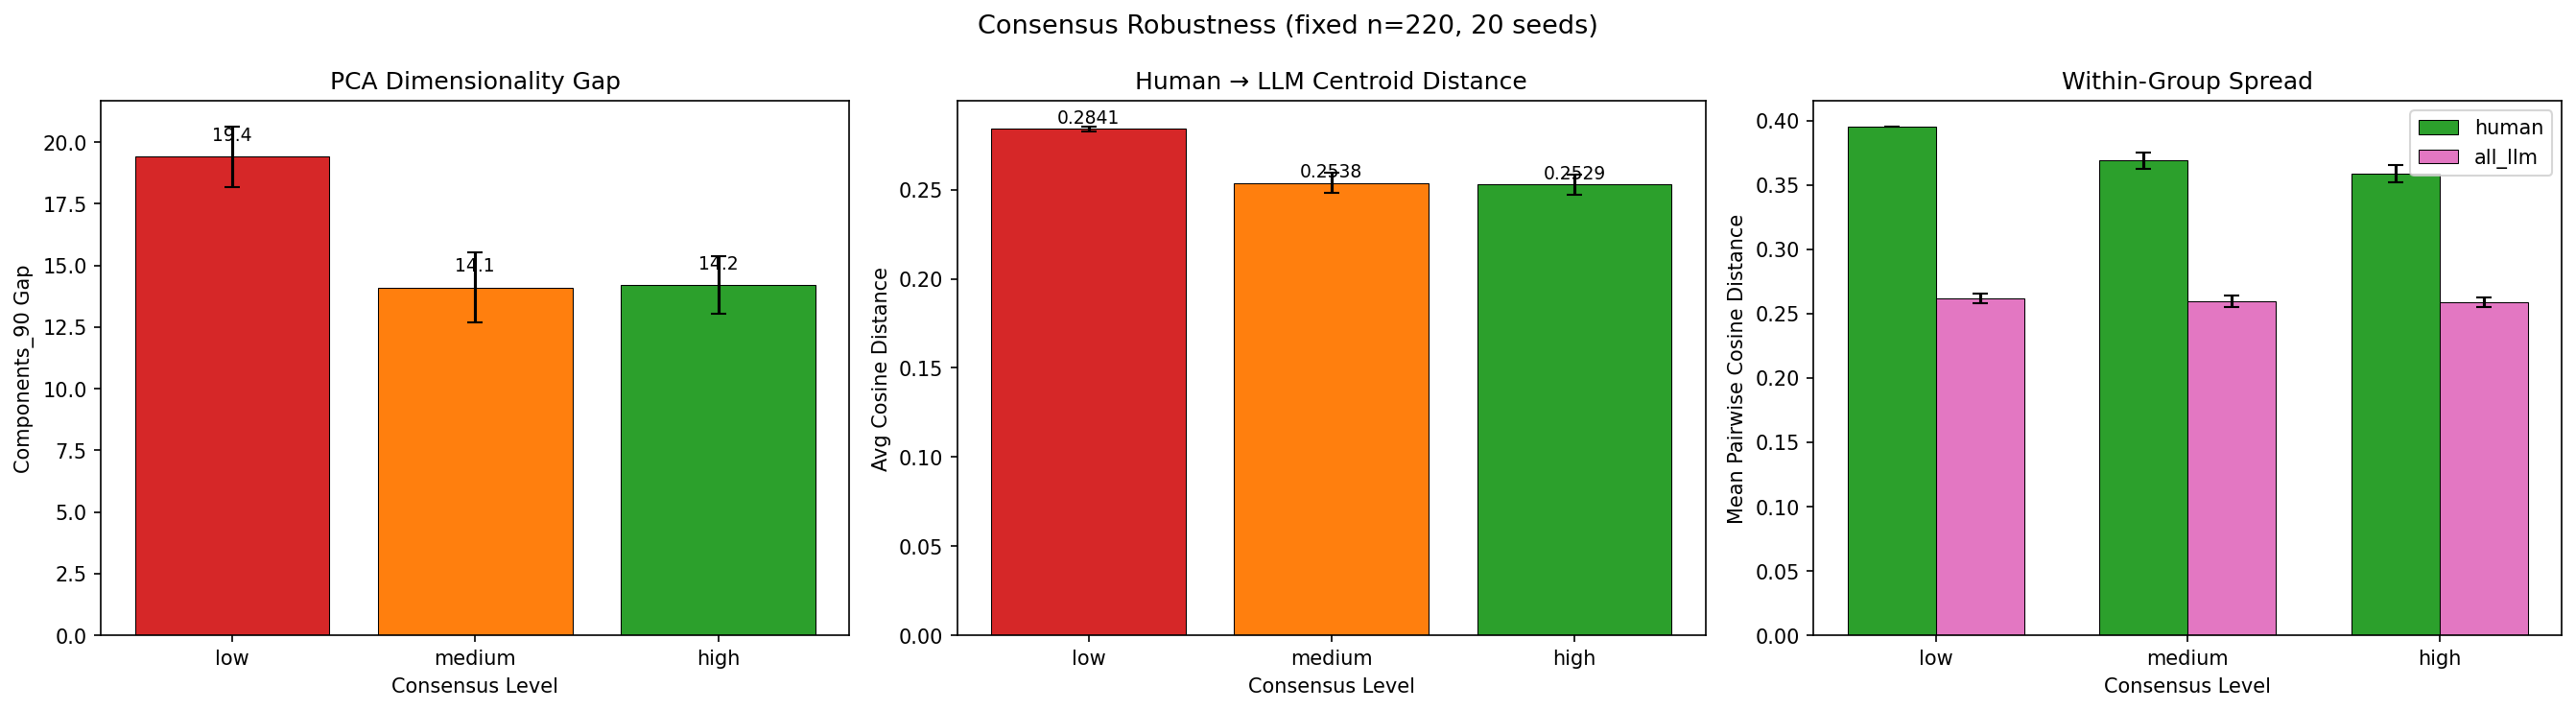
\includegraphics[width=\textwidth]{consensus_robustness_combined.png}
\caption{Three-panel consensus robustness at matched $n = 220$. Left: PCA gap persists across consensus levels. Center: human--LLM centroid distance is stable. Right: human within-group spread exceeds LLM spread at all levels.}
\label{fig:consensus_gap}
\end{figure}

\subsection{Robustness}

\paragraph{Value diversity by consensus.} The frequency distortion from Layer 4 also persists across consensus levels. At matched $n = 220$: low-consensus dilemmas yield 39 unique values ($H = 4.27$ bits), medium-consensus 73 values ($H = 4.41$), high-consensus 156 values ($H = 4.24$). Rare values like Freedom of speech appear at all consensus levels (0.5\% low, 0.3\% medium, 0.3\% high), confirming the frequency distortion is not driven by a particular type of dilemma.

\subsection{LLM Inter-Model Convergence}

Per-dilemma LLM cosine distance correlates negligibly with community agreement (Pearson $r = -0.059$, Spearman $\rho = -0.062$; both $p < 0.0001$, $n = 10{,}823$). Despite statistical significance due to large $n$, the effect size is negligible: LLMs produce the same degree of inter-model convergence whether a dilemma is morally clear-cut or genuinely contested.

\begin{figure}[H]
\centering
\includegraphics[width=0.8\textwidth]{llm_convergence_vs_consensus.png}
\caption{LLM inter-model cosine distance vs.\ consensus level. A diverse panel should show higher distance (more disagreement) on controversial dilemmas; LLMs do not.}
\label{fig:convergence}
\end{figure}

A genuinely diverse panel of moral reasoners should show more disagreement on contested cases. The seven LLMs studied here, despite different architectures and training data, maintain essentially constant inter-model agreement across the full spectrum of moral controversy (Figure~\ref{fig:convergence}). This uniformity is consistent with shared training biases producing convergent moral representations regardless of the specific model.

%% ============================================================================
\section{Layer 6: Categorical Analysis Is the Wrong Tool}
%% ============================================================================

Layers 1--5 use continuous geometric analysis (PCA, cross-projection, residual decoding). An alternative approach---exemplified by Russo et al.---treats moral values as discrete categories and measures diversity by counting which categories are used. Layer 6 tests whether this categorical lens is appropriate for the underlying data.

\paragraph{Method.} We apply $k$-means clustering at two levels: (1) to the 324 Kaleido value label strings (embedded with Sentence-BERT \texttt{all-MiniLM-L6-v2}, PCA-reduced to 50 dimensions), and (2) directly to the 227,323 rationale embeddings in Kaleido space (PCA-reduced to 100 dimensions). At each level, we sweep $k = 10$ to $200$, computing silhouette score and gap statistic (with PCA-preserving null). For the rationale embeddings, we compute per-source effective cluster count (clusters with $\geq 1$\% of a source's rationales), Shannon entropy, and top-5 concentration. We test both joint clustering (all sources in a shared PCA space) and per-source clustering (each source in its own PCA space) to diagnose sample imbalance artifacts. Silhouette scores on the 227K-point rationale matrix use a 10,000-point subsample.

\subsection{Value Label Clustering}

To test whether the 324 Kaleido value labels form discrete categories---a prerequisite for any taxonomy-based approach---we embed them with Sentence-BERT (\texttt{all-MiniLM-L6-v2}), PCA-reduce to 50 dimensions, and cluster with $k$-means. This also addresses the near-synonym problem from Layer 4: many of the 324 raw value strings are variants of the same concept (e.g., ``Family harmony'' vs.\ ``Family unity'').

\begin{figure}[H]
\centering
\begin{subfigure}[b]{0.48\textwidth}
    \includegraphics[width=\textwidth]{effective_clusters_by_k.png}
    \caption{Effective clusters used per source vs.\ $k$.}
    \label{fig:eff_clusters_k}
\end{subfigure}
\hfill
\begin{subfigure}[b]{0.48\textwidth}
    \includegraphics[width=\textwidth]{silhouette_by_k.png}
    \caption{Silhouette score vs.\ $k$.}
    \label{fig:sil_k}
\end{subfigure}
\caption{Value label clustering across $k$. (a) Both human and all-LLM track together, using 52--60 effective clusters at $k = 60$. (b) Silhouette scores range from 0.11 to 0.19---poor cluster quality throughout.}
\label{fig:value_clusters}
\end{figure}

Silhouette scores range from 0.11 to 0.19 across $k = 10$ to 200 (Figure~\ref{fig:sil_k})---well below the 0.25 threshold typically considered ``reasonable'' cluster structure. After collapsing near-synonyms via clustering, both sources use $\sim$52--60 effective moral concepts at $k = 60$ (Figure~\ref{fig:eff_clusters_k}), confirming the Layer 4 finding that categorical territory is shared. But the poor silhouette scores show that even this categorization is forced---the value labels exist on a semantic continuum.

\subsection{Rationale Embedding Clustering}

Clustering the rationale embeddings directly ($k$-means on PCA-reduced Kaleido embeddings, 227,323 rationales $\times$ 100 components) produces even worse results:

\begin{itemize}[nosep]
    \item \textbf{Silhouette scores}: 0.02--0.04 across all $k$ values tested (Figure~\ref{fig:rationale_sil})---essentially random assignment quality.
    \item \textbf{Gap statistic}: Monotonically increasing across $k = 20$ to $150$, never converging (Table~\ref{tab:gap}). There is no natural cluster count.
\end{itemize}

\begin{figure}[H]
\centering
\includegraphics[width=0.85\textwidth]{rationale_cluster_silhouette.png}
\caption{Silhouette score vs.\ $k$ for rationale embedding clustering. All values are well below Russo et al.'s 0.09 benchmark, indicating negligible cluster structure.}
\label{fig:rationale_sil}
\end{figure}

\begin{table}[H]
\centering
\caption{Gap statistic for rationale embedding clustering. Monotonic increase indicates no natural cluster count.}
\label{tab:gap}
\begin{tabular}{rrr}
\toprule
$k$ & Gap & Gap SE \\
\midrule
20  & 0.079 & 0.0003 \\
40  & 0.111 & 0.0003 \\
60  & 0.129 & 0.0003 \\
80  & 0.142 & 0.0003 \\
100 & 0.151 & 0.0003 \\
150 & 0.169 & 0.0003 \\
\bottomrule
\end{tabular}
\end{table}

\subsection{Joint Clustering Artifacts}

When human and LLM rationales are clustered jointly, the 20:1 sample imbalance (human = 4.8\% of the combined matrix) produces severe artifacts. Joint PCA captures only 65.5\% of human variance (vs.\ 76.9\% for LLMs), and 74\% of all human rationales concentrate in just 3 clusters that are almost exclusively human (Table~\ref{tab:joint_artifact}).

\begin{table}[H]
\centering
\caption{Joint vs.\ per-source clustering at $k = 60$. Joint clustering artificially concentrates human rationales.}
\label{tab:joint_artifact}
\begin{tabular}{lrrrr}
\toprule
 & \multicolumn{2}{c}{Joint clustering} & \multicolumn{2}{c}{Per-source clustering} \\
\cmidrule(lr){2-3} \cmidrule(lr){4-5}
Source & Eff.\ clusters & Entropy & Eff.\ clusters & Entropy \\
\midrule
Human   & 11  & 3.24 bits & 57 & 5.86 bits \\
All LLM & 57  & 5.79 bits & 58 & 5.87 bits \\
\bottomrule
\end{tabular}
\end{table}

When each source is clustered in its own PCA space, human and LLM rationales spread across nearly identical numbers of clusters (57 vs.\ 58) with nearly identical entropy (5.86 vs.\ 5.87 bits). The apparent human concentration in joint clustering is entirely an artifact of the minority group being forced into a cluster structure optimized for the majority.

\begin{figure}[H]
\centering
\includegraphics[width=\textwidth]{rationale_cluster_joint_vs_persource_entropy.png}
\caption{Cluster entropy: joint (left) vs.\ per-source (right) clustering. Joint clustering artificially depresses human entropy; per-source clustering shows human and LLM entropy are nearly identical.}
\label{fig:joint_vs_persource}
\end{figure}

\subsection{Why PCA Captures What Clustering Misses}

The continuous geometric analysis in Layers 1--5 captures structure that categorical analysis cannot detect:

\begin{itemize}[nosep]
    \item The \textbf{value diversity gradient} (Layer 3) is a smooth, continuous relationship across all 10,826 rationales---it would be invisible through a categorical lens that assigns each rationale to one cluster.
    \item The \textbf{cross-projection asymmetry} (Layer 2) measures asymmetric overlap between continuous distributions---it has no categorical analogue.
    \item The \textbf{dimensionality gap} itself (Layer 1) measures how many independent directions of variation exist, regardless of whether those directions form discrete clusters.
\end{itemize}

The moral value space is genuinely continuous. PCA respects this structure; clustering fights it.

%% ============================================================================
\section{Discussion}
%% ============================================================================

\subsection{The Logical Structure}

The six layers form a deductive chain. Layer 1 establishes the geometric fact: human rationale embeddings occupy 35--41\% more dimensions than LLM embeddings. Layer 2 shows the gap is asymmetric---human principal components explain most LLM variance but not vice versa, indicating the LLM distribution sits inside the human distribution rather than beside it. Layer 3 qualifies the residual stream using Kaleido's decoder, proving the extra dimensions encode genuinely diverse moral values with a nearly monotonic gradient ($r = 0.935$), confirmed independently by a general-purpose encoder. Layer 4 inventories the frequency distortion: LLMs share 84\% of the human moral vocabulary but compress the tail, with 26 values completely absent and rare values underrepresented by up to 120$\times$. Layer 5 shows the compression is structural---it persists uniformly across consensus levels and LLMs do not adapt their diversity to the difficulty of the moral question. Layer 6 provides methodological justification: the moral value space resists categorical analysis because it is fundamentally continuous, and the continuous geometric tools of Layers 1--5 are the right instruments for this space.

\subsection{Limitations}

Several caveats bound our conclusions:

\begin{enumerate}[nosep]
    \item Approximately 30\% of the surface-level text differences between poorly-captured and well-captured human rationales are stylistic (Reddit slang, profanity). The value diversity gradient is measured via decoded moral labels rather than surface text, and 82$\times$ gaps in specific values cannot be explained by profanity, but the exact decomposition of moral-vs-stylistic signal remains approximate.
    \item Each dilemma has one human rationale (the top Reddit comment), meaning this study measures \emph{across-dilemma} diversity, not within-dilemma plurality.
    \item Kaleido-XL was trained on ValuePrism, whose value annotations were generated by GPT-4 (91\% human-approved). This could bias the embedding space toward GPT-4's moral ontology. The SBERT replication mitigates but does not eliminate this concern.
    \item The models tested (GPT-3.5, GPT-4, Claude, Bison, Gemma, Mistral, Llama) are 2--3 generations old. More recent models may exhibit different diversity profiles.
    \item The low-consensus bucket contains only 220 dilemmas, limiting statistical power for that stratum.
    \item All findings are specific to AITA-style everyday moral dilemmas and may not generalize to other moral reasoning contexts.
\end{enumerate}

\subsection{Implications}

If LLMs are deployed as moral reasoning aids, content moderators, or ethical advisors, their outputs will systematically underrepresent the diversity of human moral perspectives. This underrepresentation is not random---it specifically affects rare values (Freedom of speech, Independence, Self-defense), culturally grounded reasoning, and the situational specificity that characterizes real human moral deliberation. The compression is structural, not a failure mode specific to controversial cases, and it is invisible to categorical analysis methods. Efforts to improve LLM moral reasoning diversity should focus not on the dominant moral framings (which LLMs already capture well) but on the long tail of moral values that define genuine moral plurality.

\end{document}
